\documentclass{llncs}
\usepackage{color}
\usepackage{graphicx}
\usepackage{listings, tikz, xcolor}
\usepackage{bold-extra}
\usepackage{subfig}
\usepackage{enumerate}
\usepackage{courier}
\usepackage{syntax}
\usepackage{hyperref}

\begin{document}


\title{A framework for component integration}

\author{Kardelen Hatun \and Arnout Roemers \and Christoph Bockisch \and Mehmet Ak\c{s}it}
\institute{TRESE, University of Twente \\7500AE Enschede \\The Netherlands \\
\url{http://www.utwente.nl/ewi/trese/}\\
\email{ \{hatunk,c.m.bockisch,aksit\}@ewi.utwente.nl}
}
\maketitle

\begin{abstract}
Abstract 
\end{abstract}

\section{Introduction}
Systems are often faced with new requirements for adding new functionality or updating what is already there. 
A preferred way of extending or updating system behavior is through adding components. 
A software component can be described as a self-contained entity with well-defined interface and functionality. 
Components can be plugged into target systems to extend the system with their provided functionality.
The target system contains data about the state of the system which is required by the component. 
In order to establish the data flow, connections should be made between the system and the component; this operation is usually referred as component integration or component binding. 

Depending on the extensibility of the software architecture this task can be very difficult. 
In large software systems, traditional middleware approaches such as CORBA, DCOM or JRMI can be used to manage the complexity introduced by inter-component dependencies. 
These middleware solutions are geared towards providing built-in support for widely-used technologies and offer little support for customization. 
For smaller systems, using such software can be inefficient, since they are intended to be used for component integration in enterprise software and their adoption is itself complex and requires effort. Therefore, for such systems component integration is manually implemented. Component integration is trivial when the target system and the component have a common interface. However in most cases the integration introduces the requirement that the interfaces should be made compatible with each other to make the final system functional.


This is a known problem and its solution is captured in the \emph{adapter pattern} (cite Gamma). 
Typically adapters are tailored for a given integration. 
The complexity of the adapters depend on the complexity of the structures they adapt from and to. 
For a simple type conversion between classes with small number of fields that have primitive types, the adapter is not very complex and it can be easily maintained when either of the classes change. 
However for classes which contain fields of other types, which themselves are composite, the adapter implementation becomes more complex.
This results in adapter implementations that hide the \emph{ugly} adaptation code, which are fragile against software evolution and not reusable. 

In the end component integration boils down to instance-level dependencies. 
Hence another important step of integration is assigning the data values to the relevant fields.  
Keeping the system and the components loosely coupled is an important principle of component-based design. 
Dependency injection (DI) (cite fowler) is a lightweight method for keeping modules loosely coupled by delegating the creation of concrete objects to so-called \emph{injectors}. This approach allows a highly customizable and an agile way of creating dependencies, while maintaining loose coupling.

In this study we introduce a light-weight component integration framework, which is based on composable integration modules. 



which incorporates aspect-oriented programing, dependency injection and integration structures that are influenced by enterprise integration patterns (cite Hophe). 
Our framework is especially useful when the system or the component does not implement predefined interfaces and must be manually bound together. 
We automate the adaptation process by exploiting the type hierarchies and provide checks and context-relevant messages for correct integration.


\section{The Framework}

\begin{figure}
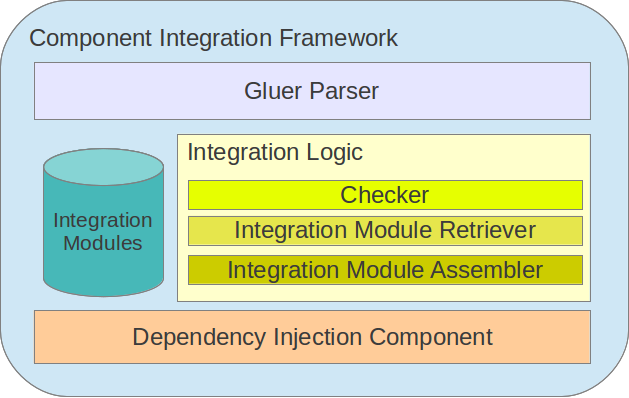
\includegraphics[width=0.75\textwidth]{images/integrationframework.png}
\caption{An abstract view of the integration framework}
\label{fig:main}
\end{figure}

In figure~\ref{fig:main} an abstract view of the framework is shown. The framework consists of several components. 

\subsection{The Gluer Language}
We have designed a small language which is used to declare structures that will be bound via our framework. 

\begin{enumerate}
\item the gluer syntax
\item new, single, method return semantics
\item splitter aggregator syntax and semantics
\item instance pointcut integration, syntax and semantics, limitations?
\end{enumerate}

The \textsf{gluer parser} is responsible for parsing associations and performing syntax checks. Once the where field (target of the injection) and what object (the object to be injected) are parsed, the what objects are passed to the integration logic to be processed.

\subsection{Integration Logic}
The integration logic is responsible for wrapping the what objects with appropriate adapters to be injected to where field. 
The what objects may need to be preprocessed before adaptation, a what object can be split into different objects (one-to-many) or multiple what objects can be aggregated to a single object. 
These operations are done automatically by the integration logic. Figure~\textbf{ref} shows the flowchart of operations that take place for finding splitters and aggregators for objects.

\textbf{flowcharts for splitter and aggregator}

\subsection{Integration Modules}

The integration modules are composable 

\subsubsection{Splitters}
\begin{enumerate}
\item how are they defined; regular classes with @Splitter annotation, They should implement the ISplitter interface which comes with the split(Object) method
\item How are they registered, we may need some meta information
\end{enumerate}

\subsubsection{Aggregators}
\begin{enumerate}
\item how are they defined; regular classes with @Aggregator annotation, They should implement the IAggregator interface which comes with the aggregate(List --Object--) method
\item How are they registered, we may need some meta information
\end{enumerate}

\subsubsection{Adapters}
Once the structural mapping is done, the resulting object(s) should be adapted to be injected. This step is also automated\ldots

\textbf{The flowchart from Arnout about adapter retrieval}

\subsubsection{Adapter Resolution}
Precedence rules

Informative error messages



\subsection{Instance Pointcuts}
\textbf{Recycle text from instance pointcuts paper}

The injection framework is based on creating new object. What if we would like to inject specific objects which already exist in the system. Then we need a way to select these objects. We have designed and implemented instance pointcuts which allow the selection of objects of a certain type according to events in their life-cycle. Instance pointcuts can be used on their own, also they are seamlessly integrated with the adapter injection framework. 
Semantics
For an instance pointcut which collect objects that are applied a discount, “discountedItems” we can use the following association.

\texttt{associate listfield with discountedItems}


if the type of the instance pointcut is incompatible with the type of the list field, then each object in the “discountedItems” will be wrapped with the appropriate adapter.  This association ensures that the \texttt{listfield} will stay updated according to the discountedItems instance pointcut. (what about type erasure? How do we know what type of object does \texttt{listfield} hold?, Java ClassMate Library)

It is also possible to associate a non-list with an instance pointcut then the behavior will be updating the associated field with the object that is added the latest to the instance pointcut set. 
Note that add instance pointcut integration also adds dynamic behavior to the injection framework, since instance pointcuts set is dynamically changing throughout the execution.
Instance pointcuts are also useful in filtering objects, due to their event based definition. It can select object that only participate in a specific event, which allows usage-based adaptation. 

\subsubsection{Usage-based adaptation}
Instance pointcuts allow objects to be selected according to how they are used. Integrated with the adapter injection framework, this allows wrapping objects based on their uses in the system.
Implicit content change case
Some methods can change the contents of an object, which may require the object to be handled later in its life cycle. These changes may not necessarily require creating an object of different type.
Example: A file object is passed to the addHeader() method, this method appends a header at the beginning of the file contents. This method changes the content of the file. This is an implicit event. The type of the object is still File, so how will the system know if this file has a header or not, if a flag is not present? Instance pointcuts can bookkeep such objects.

\end{document}